\begin{figure}[ht]
    \centering
    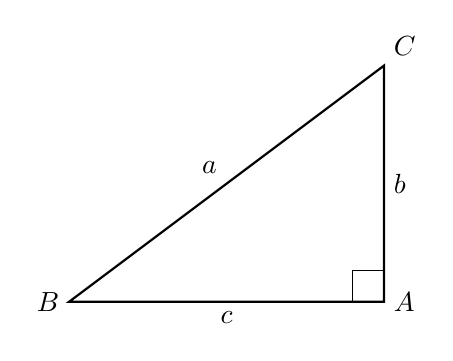
\begin{tikzpicture}
    % Pontos do triângulo
    \coordinate (B) at (0,0);
    \coordinate (A) at (4,0);
    \coordinate (C) at (4,3);

    % Lados do triângulo
    \draw[thick] (B) -- (A) -- (C) -- cycle;

    % Marcação do ângulo reto em A
    \draw (A) ++(-0.4,0) -- ++(0,0.4) -- ++(0.4,0);

    % Nome dos vértices
    \node[right] at (A) {$A$};
    \node[left] at (B) {$B$};
    \node[above right] at (C) {$C$};

    % Lados a, b, c
    \path (B) -- node[above left] {$a$} (C);
    \path (A) -- node[right] {$b$} (C);
    \path (A) -- node[below] {$c$} (B);

    \end{tikzpicture}
    \caption{Triângulo retângulo.}
    \label{fig:triangulo-retangulo}
\end{figure}
